\documentclass[11pt,a4paper]{article}
\usepackage[utf8]{inputenc}
\usepackage[T1]{fontenc}
\usepackage[english]{babel}
\usepackage[margin=3.5cm]{geometry}

\usepackage[hidelinks]{hyperref}
\usepackage{graphicx}

\title{SnelSLiM User Manual}
\author{Bert Van de Poel}
\date{13 August 2020}

\begin{document}

\maketitle

\tableofcontents

\newpage

\section{Introduction}

SnelSLiM is a corpus linguistics tool to make it possible to quickly and easily perform Stable Lexical Marker Analysis (a form of keyword analysis) and gain insight into corpora. This manual tries to guide users when using snelSLiM for the first time. It presumes the user has an account on an existing online installation of the application.

To install snelSLiM, it is advised to point the system administrator of your research group, department, faculty or company towards the installation instructions on \url{https://github.com/bertvandepoel/snelSLiM/blob/master/INSTALL.md}. While of course this manual can be read without having access to a working installation and account, it makes more sense to follow along online. 

If you are looking for details concerning the academic publications on Stable Lexical Marker Analysis (henceforth SLMA), please refer to the ``What is SLMA?'' help page of your installation. If you are looking for details on and formulas of the statistics used within snelSLiM, please refer to the ``What statistics are used?'' help page of your installation. Examples of corpus formats, as well as an FAQ are also available through help pages.

More details on the different libraries used can be found in the acknowledgements file on \url{https://github.com/bertvandepoel/snelSLiM/blob/master/ACKNOWLEDGEMENTS} or on the about page of your installation.

If you are an advanced user wishing to use the binaries behind snelSLiM as command line tools, please refer to the help information printed by the preparser and analyser binaries when executed without parameters.

\section{Selecting corpora}

After logging into your installation of snelSLiM, the main form is displayed, ready to commence a Stable Lexical Marker Analysis. 

\centerline{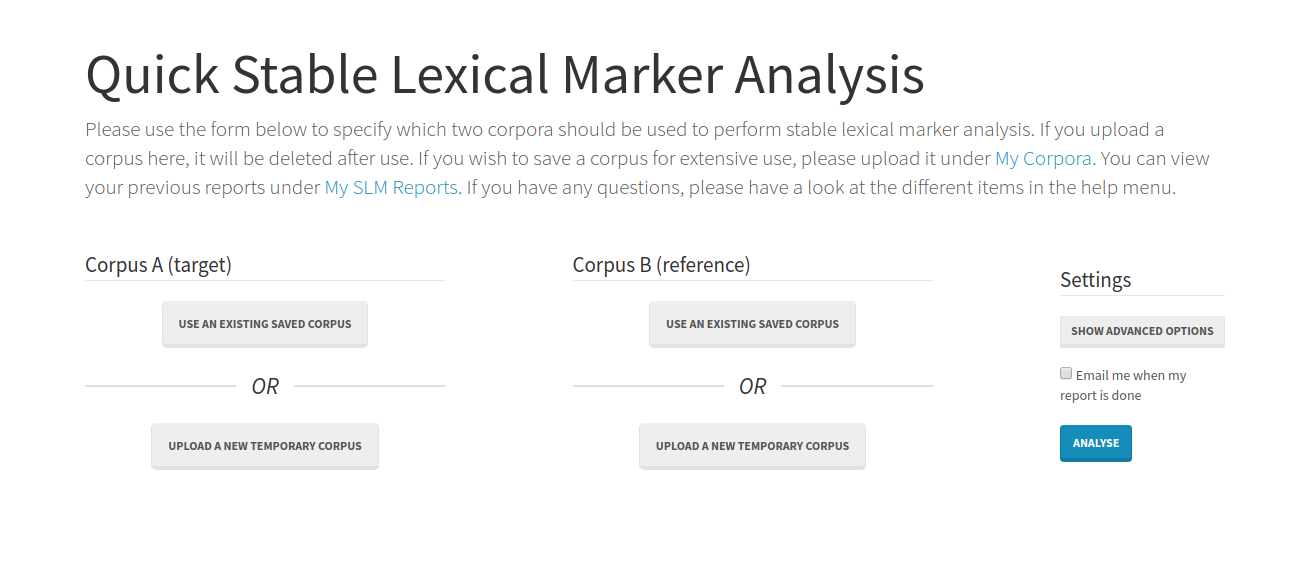
\includegraphics[width=\textwidth]{images/form.png}}

For both the target and the reference corpus, you can either select an existing corpus or upload a new one. 

\subsection{Using saved corpora}

Depending on the size of your corpus and the speed of your connection, it may take quite a while to upload a corpus. When performing SLMA with different settings or with one of the two corpora staying identical, it can therefore save a lot of time to save it within snelSLiM. This can also save some extra processing time since the corpus is stored in a preparsed format ready for SLMA.

There are two forms of saved corpora: global corpora and personal corpora. After clicking on ``My Corpora'' in the top menu bar, you can view the personal corpora you've saved, as well as delete and add corpora. The process to add corpora here is discussed in the next section. Personal corpora are only available from your account. Other users can't see or use them.

\centerline{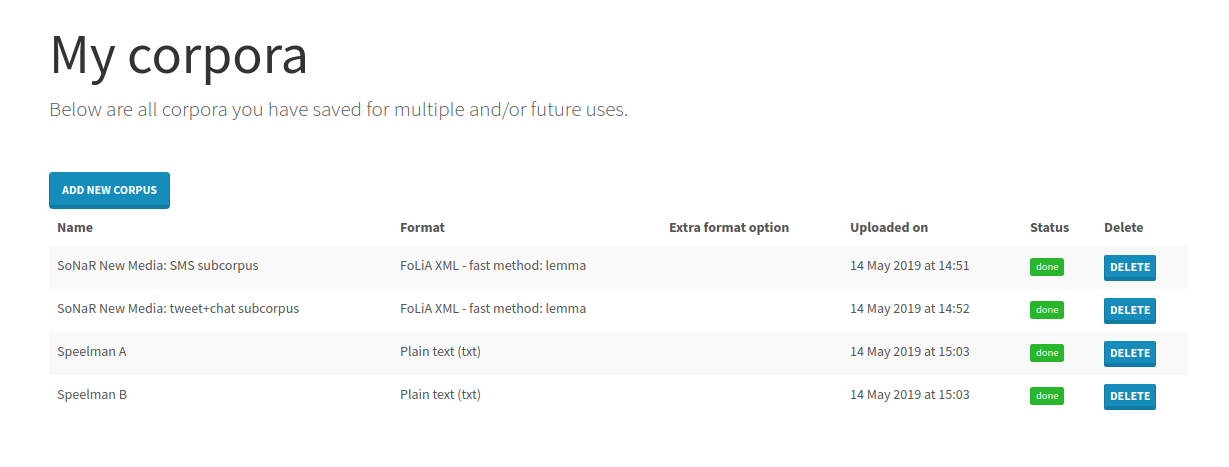
\includegraphics[width=0.9\textwidth]{images/mycorpora.png}}

Global corpora are available to every user of your installation. They can be useful if for example your research group has some corpora several researchers are working on, or to supply some good reference corpora representing certain languages or certain media or registers. 

Admin users can manage these global corpora on their ``My corpora'' page, as well as make their personal corpora global.

\centerline{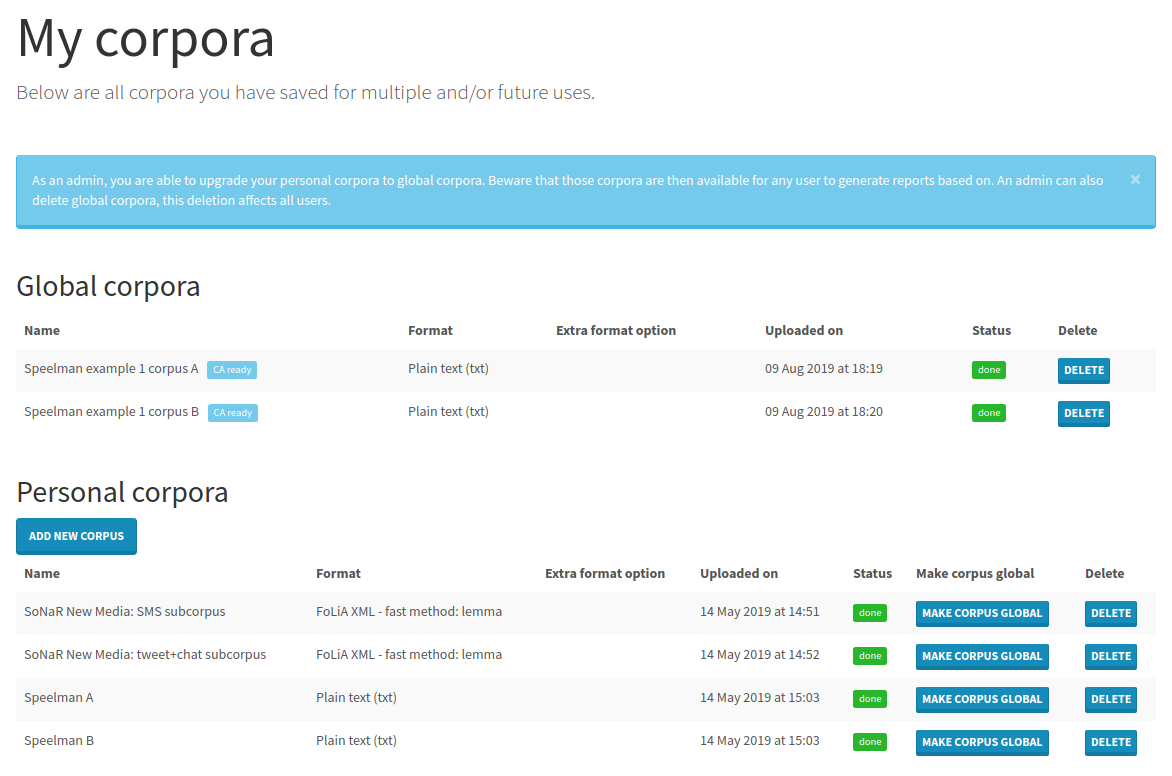
\includegraphics[width=0.9\textwidth]{images/admincorpora.png}}

Within the selection screen of the main form, displayed after clicking on ``Use an existing saved corpus'' for the target and/or reference corpus, global corpora (if there are any) are displayed before personal corpora. Since both parts of this list can potentially get quite large, a search function is available to look for parts of the name of the corpora. Once the desired corpus has been found in the list, it can easily be selected by clicking on it. It will remain selected until another corpus in the same list is clicked, or the back button is pressed for that corpus.

\centerline{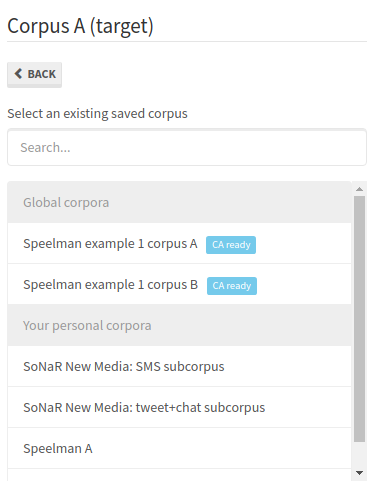
\includegraphics[width=0.4\textwidth]{images/corpusselect.png}}

\subsection{Uploading new corpora}

If the corpus you wish to analyse is not available yet, it can either be uploaded as a new temporary corpus on the main form or as a new saved corpus on the ``My corpora'' page. 

Temporary corpora are only available for single use. That means they are used within the analysis they are uploaded for, and then disappear. This can for example be useful when testing manually curated corpora or verifying the clean-up of a corpus.

\centerline{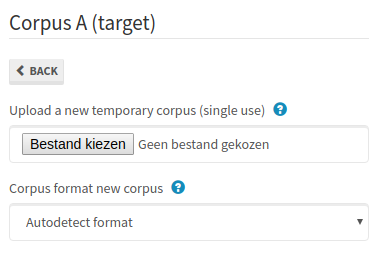
\includegraphics[width=0.4\textwidth]{images/corpusupload.png}}

The forms to upload temporary corpora or new saved corpora are fairly similar. Whether saving the corpus or just using it for a single report, you need to upload a single file. This file can be a zip, tar, tar.gz, tar.bz2 or tar.xz, but can't be several separate corpus files. Most operating systems supply an option within their file manager to create a zip file, often referred to as ``compress'' when right clicking a folder. It's important to make sure filenames are not re-used within the supplied corpus archive, since snelSLiM doesn't take into account the potentially very complicated directory hierarchy of some corpora. In case of duplicate filenames, the file is overwritten in the analysis by the last instance with that filename. In most cases that is not what you want. It's also important to make sure only actual corpus files are included, and no documentation, metadata files or other miscellaneous files. Finally, the supplied corpus should only contain corpus files in a single format. Most corpora are either supplied in a single format already or have the formats separated in different folders, make sure to check this before uploading. If incorrect files or incorrect formats are parsed, they will most probably show up as files containing 0 words, which will trigger a warning and will obviously invalidate the results of your analysis.

After preparing your corpus file and selecting it using the file browser, you have the option to indicate the corpus format. By default, this dropdown has the autodetection feature selected. The autodetector of snelSLiM is able to recognize the following formats:

\begin{itemize}
    \item FoLiA XML
    \item DCOI XML
    \item Alpino XML
    \item TEI XML (BNC/Brown Corpus variant)
    \item XCES GrAF (used for OANC and MASC)
    \item PRAAT TextGrid
    \item Corpus Gysseling format
    \item Corpus Eindhoven format
\end{itemize}

When one of these formats is detected, it is presumed the user wants the lemmas and not the bare words to be extracted for analysis. Beyond detecting these formats, the autodetector can indicate it doesn't recognise the files, it detects several formats, it recognised some files but not all those that were tested, or it might indicate it recognises the corpus as potentially being in a format that requires user input. In the last case, it might be a CoNLL tab seperated values, where a user would have to supply the index of the column to extract words/lemmas from, or an unknown XML format, in which case a user could supply a simple XPath query to make it possible for snelSLiM to start the analysis.

A very common corpus format that cannot be autodetected is a simple plain text corpus. In case of a plain text file, no form of metadata, annotations or tagging is added, but the bare text is supplied as is. A user can easily check whether that is the format of their corpus and then change the dropdown to ``Plain text (txt)''. 

If you would like to know more about the different formats supported by snelSLiM and how to recognise them, please refer to the help page on corpus formats.

For a temporary corpus, the file and the format are the only options, but for a saved corpus there are one or two more. For a regular user, the form for a new saved corpus also asks for a name for the new corpus. Since filenames can sometimes contain abbreviations, or there might be several versions of the same corpus, it's worth considering adding the full name and all relevant details such as version number or subcorpus selection parameters to the corpus name.

\centerline{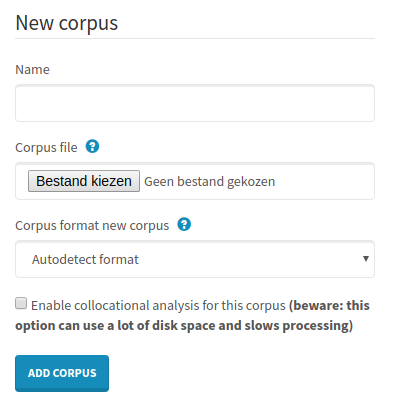
\includegraphics[width=0.4\textwidth]{images/uploadmycorpora.png}}

If your account has been given special permission to use more resources, you may be able to tick a checkbox to enable collocational analysis for the corpus you are uploading. This uses a lot more disk space, since the corpus can't be reduced solely to frequency lists, but full texts have to be preserved.

\section{Analysis settings}

After selecting existing corpora, preparing new files to be uploaded, or both, you can proceed to immediately request an analysis. However, beyond the email notification option that's shown by default, there are several other options to tweak your analysis by clicking the ``Show advanced options'' button.

\centerline{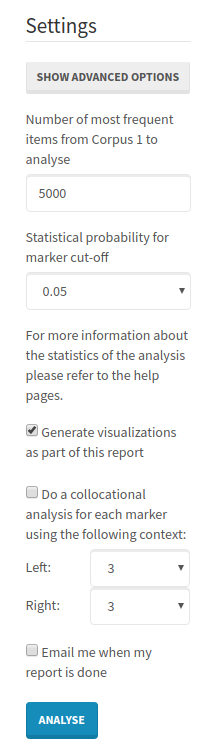
\includegraphics[width=0.2\textwidth]{images/advancedsettings.png}}

Since corpora can get quite large and contain many unique words, not every unique word is necessarily tested as a potential stable lexical marker. Instead only a certain number of most frequent items are analysed. This can be changed by the user based on the size of the corpora, their experience with the corpora, and previous results where perhaps every tested item was a marker and therefore a broader analysis is required. The system administrator can, while installing the application, impose a limit to prevent egregious usage of resources. 

After the number of most frequent items, there's a dropdown to controle the statistical probability cutoff used in SLMA. The percentage represents the statistical probability of an accurate result. Keep in mind that as many calculations are performed, the default is 99.9\% here and not 95\% as is common with other methods. More detailed information about the statistics behind this option is available on the help page ``What statistics are used?''.

Next is a, by default ticked, checkbox for visualisations. If you do not desire any visualisations in your report, you can disable this option. This will result in no treemap or scatter plots being displayed, as well as the detailed file reports being unavailable. Depending on the corpus size and the amount of requested frequent items, this may have a noticeable impact on analysis speed.

Second to last are the options for collocational analysis. First of all a checkbox to perform collocational analysis if available. If an existing A corpus is not preparsed for collocational analysis (missing the ``CA ready'' label), or the user uploads a new temporary corpus but lacks the correct account permissions to preparse that corpus for collocational analysis, a friendly message will be added to the report and CA will not be performed. It can be useful to disable CA when you are not planning to use its results as it will save time and resources. After the checkbox, the search windows (left and right) can be specified. This indicates how many words to the left and/or the right from a marker collocates should be searched and checked for. The window is counted exclusively, so the numbers do not include the marker itself. For more details on the techniques used to perform collocational analysis, please refer to the help page ``What statistics are used?''.

Finally, there's the email notification option. This is the only option shown by default. When working with large corpora with many files, many calculations have to be performed. This may result in an analysis not taking a few seconds but several minutes or even over an hour. In that case it's not always convenient to leave your web browser open. So you can request that snelSLiM emails you when your report is finished.

After you've finished inputting your desired settings into the form, you can press the analyse button to start the analysis. As soon as the green message is displayed your analysis has begun, you are free to close your browser tab. While you can leave it open and it will automatically refresh until your report is ready, there is no requirement to do so as soon as you've received a message the analysis is ongoing.

\section{Understanding a snelSLiM report}

After submitting a new analysis, it's available under the menu item ``My SLM Reports''. Here you can see which corpora were selected, what options were chosen, and whether the report is still processing, has encountered and error or is done.

\centerline{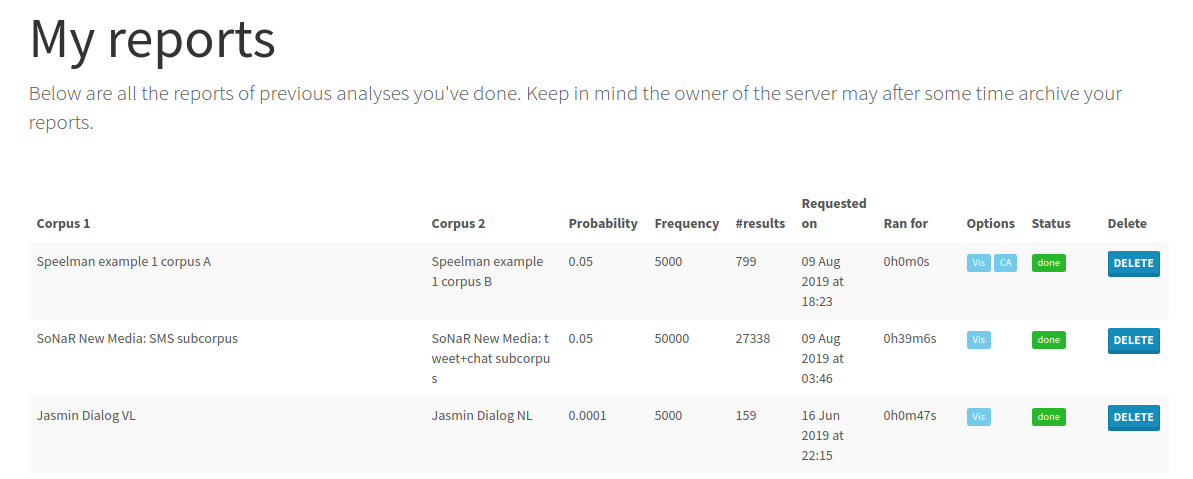
\includegraphics[width=\textwidth]{images/myreports.png}}

If a report were to encounter an error, you can view it by hovering over the red error indicator.

\centerline{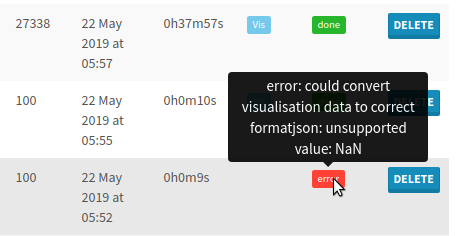
\includegraphics[width=0.4\textwidth]{images/reporterror.png}}

You can click anywhere on the line (except for the deleted button of course) to view the report. You will then first end up on the main report.

\subsection{The main report}

As long as your report is still being processed, a temporary message will be displayed. As soon as it's done, you will be greeted by ``Your report is ready'', followed by a detailed description of your report settings, some details on the processing time, and how many markers were found. 

\centerline{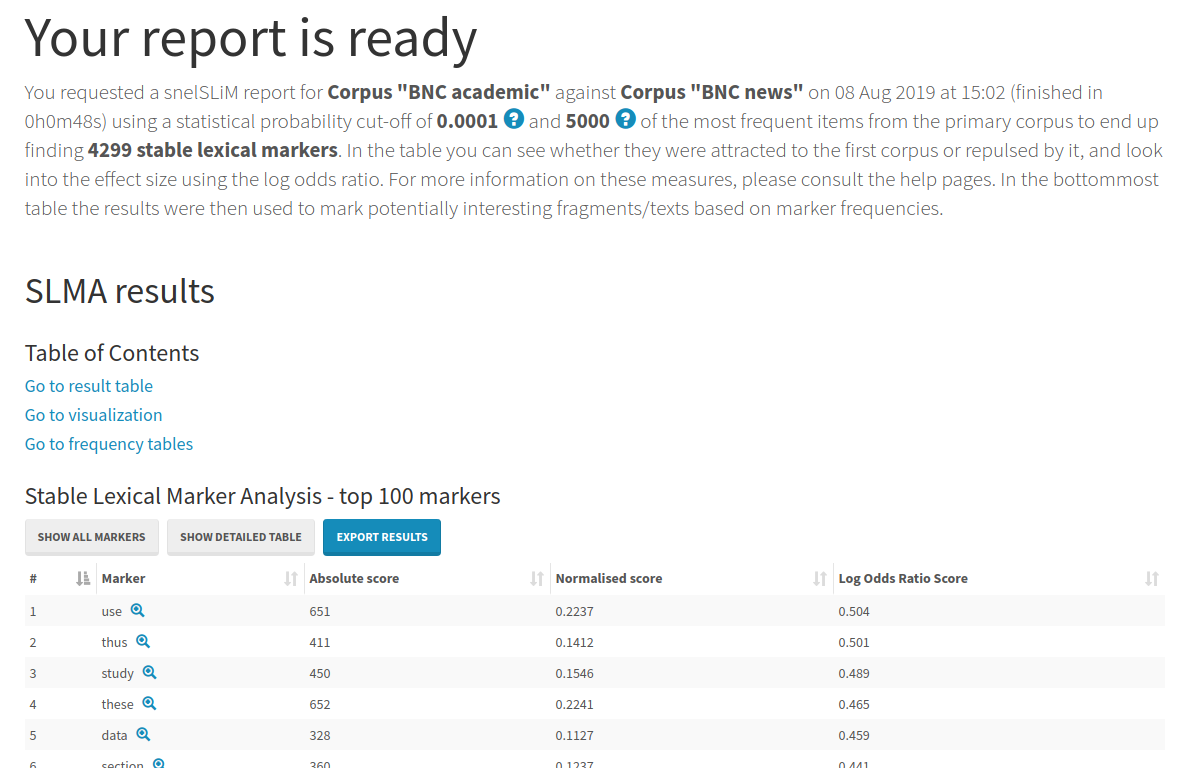
\includegraphics[width=0.9\textwidth]{images/mainreport.png}}

The page features a table of contents which makes it possible to jump to specific sections of your report. This, combined with a button on the bottom right to return to the top of the report, makes it easier to browse a report with many markers and many texts or fragments. 

By default the top 100 markers, based on the log odds ratio score, are displayed together with their absolute score, normalised score and the log odds ratio score. By pressing the ``Show all markers'' button, you can display all markers instead of the top 100 with these columns. If you press the ``Show detailed table'' button, the attraction, repulsion, lowest log odds ratio, highest log odds ratio and standard deviation are all displayed, as well as all markers. Keep in mind that both of these options result in loading quite a large table, which will take a few seconds. It's possible to sort the table by other columns than the log odds ratio score by using the arrow icons on the right side of each column header, this can also take several seconds. The ``export results'' button is discussed in the next section of this manual.

Clicking on the magnifying glass icon next to a marker opens up the detailed marker report for that marker.

\centerline{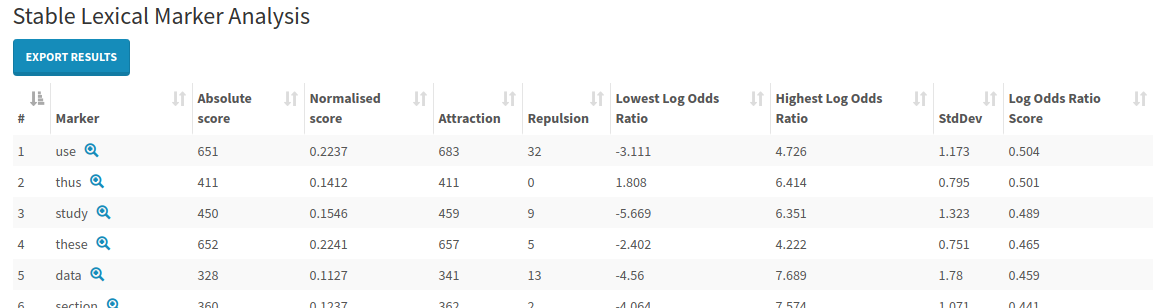
\includegraphics[width=0.9\textwidth]{images/mainreport_detailtable.png}}

After the main results table, several visualizations are available (if visualisations weren't disabled for this report) to help assess which files to inspect or which aspects of the corpora to (re)consider. First, a treemap visualisation representing the target corpus is displayed. At the top, two dropdown elements are displayed. The first gives the user the possibility to decide what the size of the blocks of the treemap elements are based on. Specifically, the number of markers in each file, the number of unique markers in the each, or one of those relative to the number of total words/lemmas in the file. The colour can be based on the total number of markers per category (being attracted or repulsed markers), or the number of unique markers per category. For a very consistent target corpus that had a very successful stable lexical marker analysis, the treeview will yield many blue files or mostly the same size. However, if some files turn up red, or there are some large inconsistencies in size, this may be interesting to investigate. For example a certain file might be an interesting outlier that features a much higher or much lower density of markers. At the same time it could also signal problems with the quality of the corpus (see Common pitfalls later in this manual).

\centerline{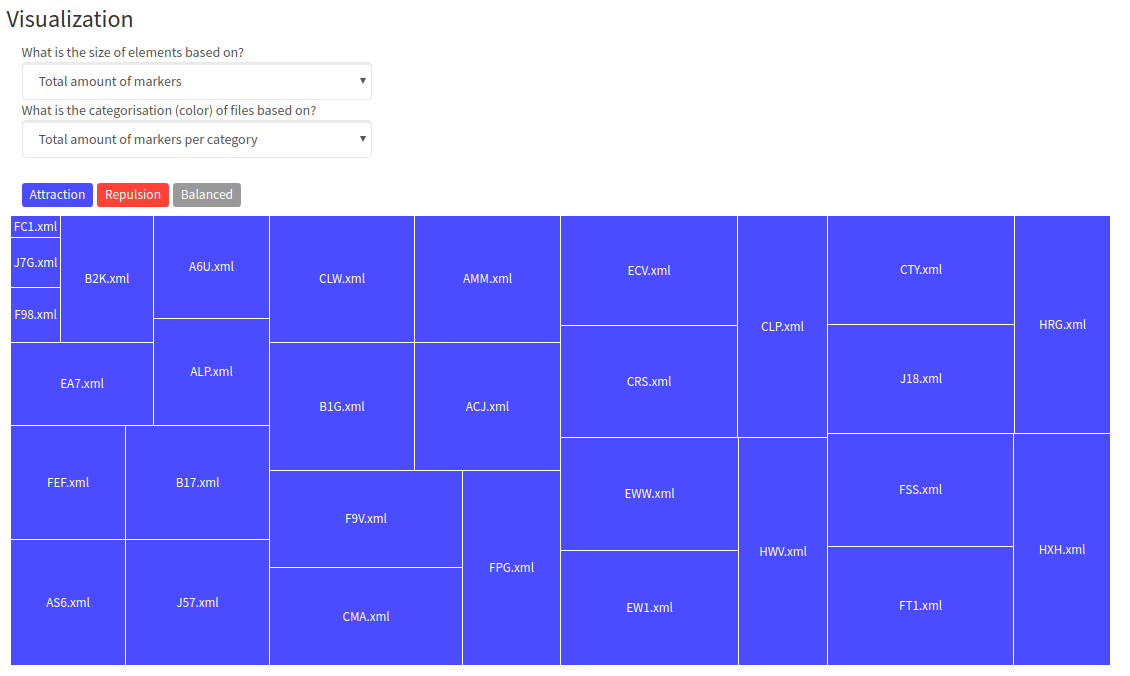
\includegraphics[width=0.9\textwidth]{images/treemap.png}}

Following the treemap visualization, the first of two scatter plots is displayed. These two scatter plots are based on representing each file as a vector of the effect sizes of markers that were attracted to that file. The first plot uses the distance between vectors to display the clustering of files. This way, it's possible to gain some insight whether the files of your corpora are diverse or rather similar in keyword distribution across files. It may also be interesting to see what specific files are outliers and whether they are for example also files that contain mostly repulsed keywords in the treemap visualization.

\centerline{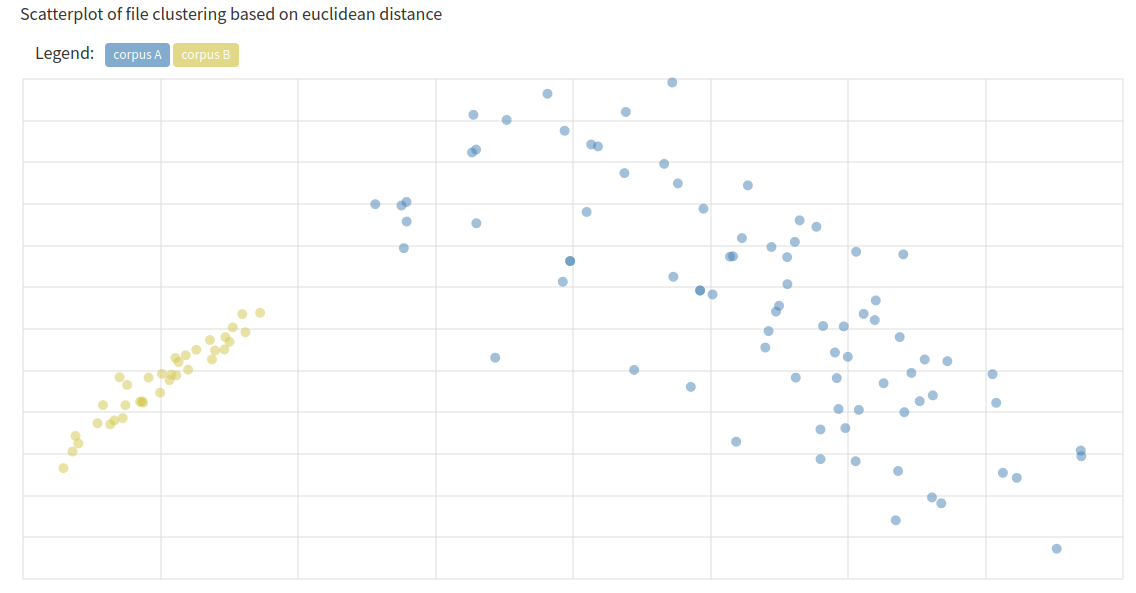
\includegraphics[width=0.9\textwidth]{images/euclid.png}}

As mentioned before, the final visualization is also based on the vectors used for the other scatter plot. While both display the clustering of files from both corpora, the second scatter plot uses a comparison with an average stereotype for each corpus. This way, it's possible to see which files are key to a corpus and which are of less importance, but also if there's potentially some file that has a great similarity to the corpus it's not part of.

\centerline{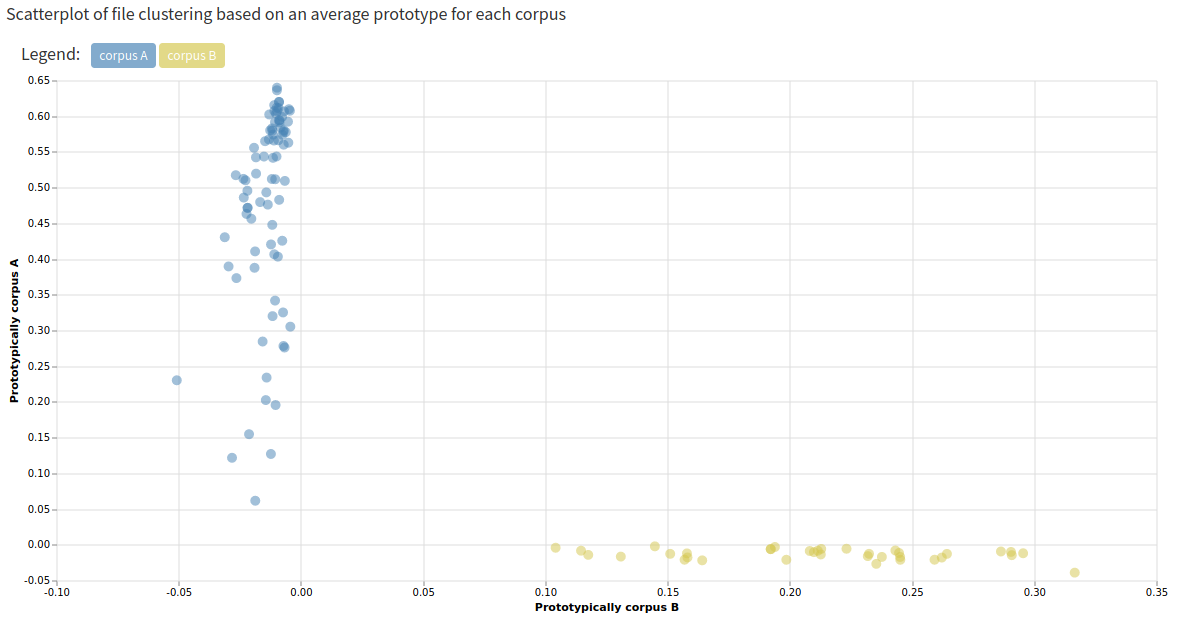
\includegraphics[width=0.9\textwidth]{images/proto.png}}

Clicking on the different elements of the treemap representing different files or any of the marks on the scatter plot opens up the detailed file report for that specific file.

Underneath the visualisations, two tables are displayed. The left table represents the files (which represent text fragments or individual texts) in the target corpus, the right table is the same but for the reference corpus. For each file, the filename, file extension and the amount of markers in the file are listed. The file extension enables users to easily see anomalies, using the sorting arrows. If visualisations haven't been disabled, icons are displayed on the target corpus table which link to the detailed file report for that file (similar to clicking on elements on the treemap).

\centerline{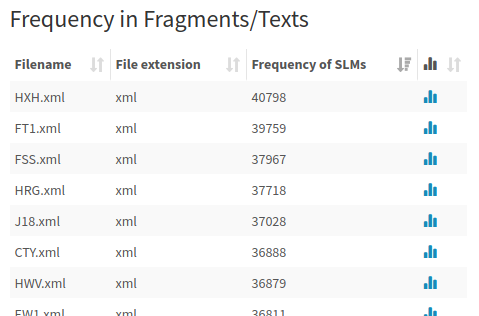
\includegraphics[width=0.6\textwidth]{images/mainreport_frac.png}}

\subsection{Exporting results}

By clicking on the ``Export results'' button at the top of the main report page, it's possible to export the main result table to many formats. Depending on whether you want to export your results for use in R, Excel, LaTeX or another tool, you can choose another export file format. To minimise the need to remove unnecessary columns, you can decide which ones you which to include. By clicking on the ``Export'' button, the file you requested will be downloaded to your computer or displayed within your browser ready to copy.

\centerline{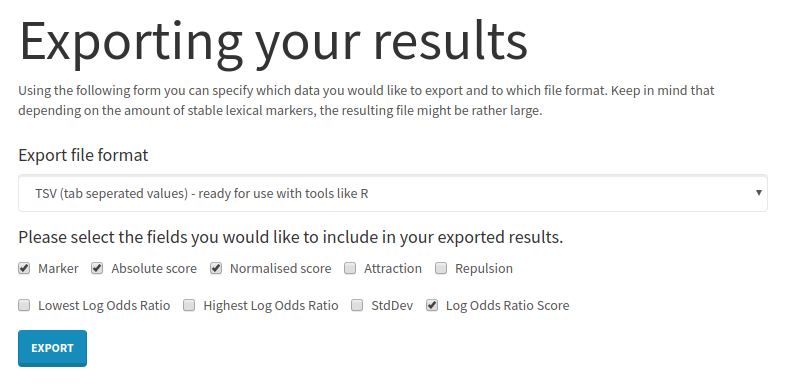
\includegraphics[width=0.7\textwidth]{images/exportresults.png}}

\subsection{Sharing reports}

Next to the ``Export results'' button, a final button ``Share report'' is available to share your report with others. There are two ways to share reports. The first is using a shareable link. Once generated, anyone with this link will be able to view the full report including all details. The link can be revoked so access is again private, it's then possible to generate a new, different shareable link. It's possible to include a shareable link as part of a publication so others are able to verify your results. A more restricted way of sharing results is to a specific user. Using the email address associated with any account on your snelSLiM instance, you can share a report to them. The user will receive and email and will by able to see the shared report on the ``My reports'' page under a separate section. Again, access can easily be revoked. A user can also opt unshare a report that was shared with them if they no longer wish to have access to it.

\centerline{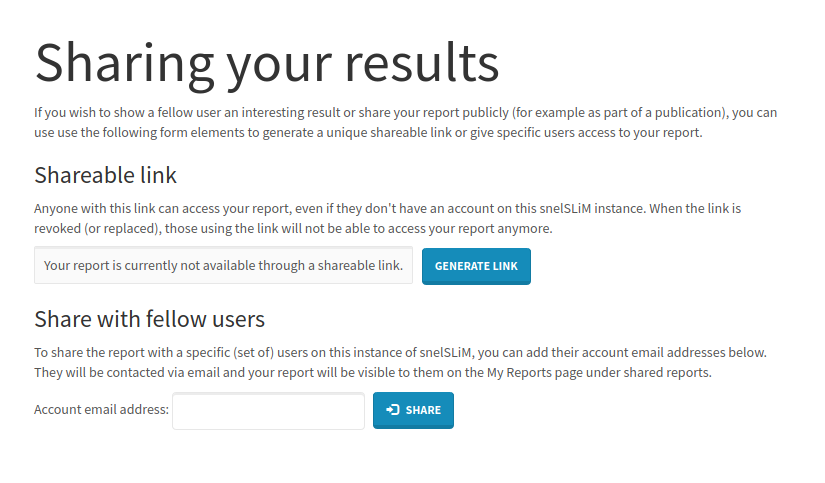
\includegraphics[width=0.7\textwidth]{images/share.png}}

\subsection{Detailed marker report}

By clicking the magnifying glass icon next to a marker in the main results table, you can open up the detailed marker report for that specific marker. This report features a short introduction with basic information about the report and the marker, including its frequency in the target corpus, its position within the frequency graph of this corpus, as well as what percentage of the corpus is represents. Afterwards, the single row for this specific marker from the main results table of the report is repeated in full detail.

On the bottom left, each file is listed that features the marker, together with its frequency. If collocational analysis was requested for this report, the collocates of the marker, together with their log Dice score, are listed on the bottom right. For more information about the statistics behind collocational analysis and log Dice, please refer to the help page ``What statistics are used?''.

\centerline{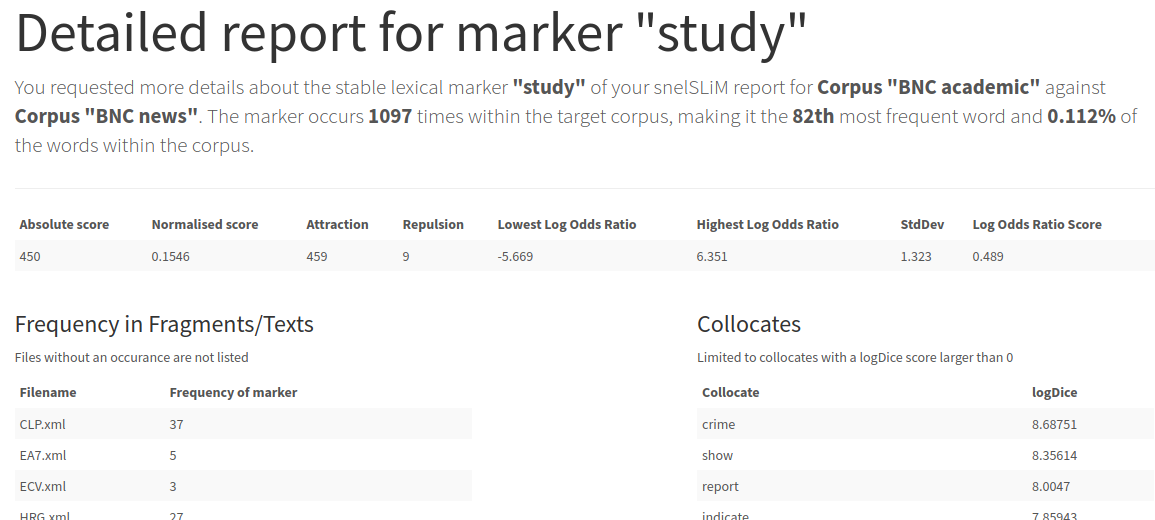
\includegraphics[width=0.9\textwidth]{images/keyreport.png}}

\subsection{Detailed file report}

By clicking on a file's element within the treemap or the graph icon in the fragment table of the main report, you can open up the detailed file report for that specific file. These reports are only available if visualisations weren't disabled. This report features a short introduction with basic information about the report and the file, including how many words and how many markers it contains, how many unique markers are featured, what percentage of the file is markers, and whether the majority of markers and unique markers are attracted or repulsed. 

After this introduction, a visualisation is shown which represents each stable lexical marker from this analysis as a single square. If it isn't present within this file, it's left blank. However, if the marker is present, it's coloured based on whether the marker is attracted, repulsed or balanced (equally as much attracted as repulsed). This visualisation makes it possible to look in more detail at files that seem to have anomalous results, as discussed in the paragraph concerning the treeview visualisation. If your analysis has a very large amount of stable lexical markers, it might be worth clicking on the visualisation to open it in fullscreen and be able to zoom using your web browser or even save it to your computer.

\centerline{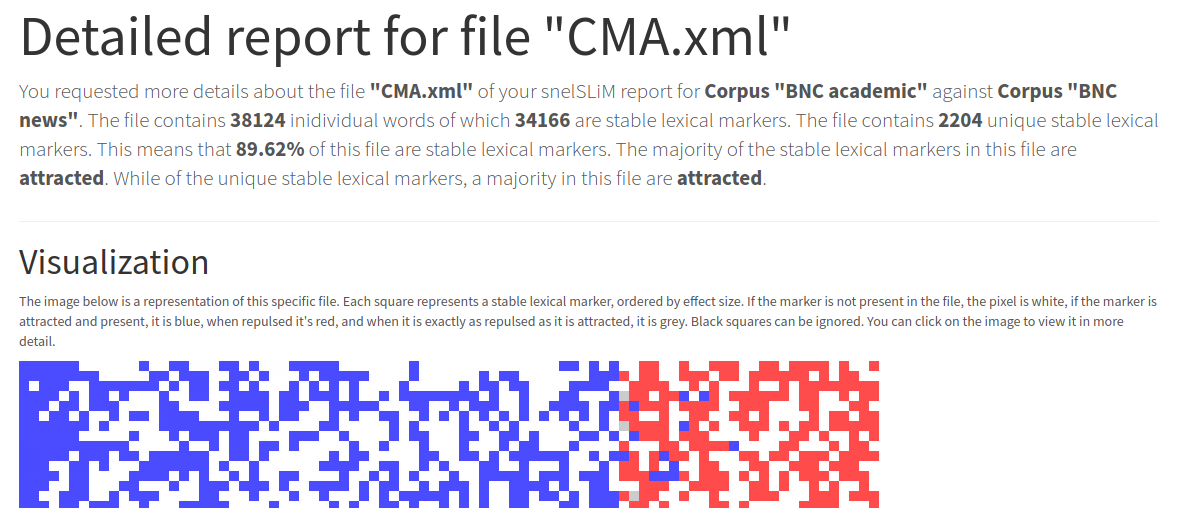
\includegraphics[width=0.9\textwidth]{images/filereport.png}}

\section{Common pitfalls}

It's important to keep in mind that inconsistent corpora or corpora that have not been cleaned up correctly, can result in anomalous analysis results. For example corpora with files that contain very few words or that contain files that cannot be parsed and therefore in the eyes of snelSLiM contain no words, can lead to strange behaviour if potential markers are very prevalent in other files. Luckily, these files are easily noticed in the treeview, resulting in great differences in element size with certain dropdown settings, and of course using the fragment table to look for low frequencies and unexpected extension. The detailed file reports can then be used to investigate these files, or you can of course open the source corpus (if available to you) on your own computer to investigate those files by hand.

SnelSLiM tries to catch the most problematic corpora by displaying warning labels next to them and by showing large warnings when analyses are performed using potentially problematic corpora. The lack of a warning however doesn't mean your corpora are necessarily of good quality.

Another potential pitfall is not considering the effect size of markers. While statistical tests are used to check if a word or lemma is potentially a marker, it doesn't necessarily have a great effect size.

Finally, it might be useful to consider changing the amount of frequent items that are analysed and the probability that's being used when the amount of results and the amount of frequent items are identical or very close. Looking into the probability is also worth your attention when there is a unexpectedly large amount of keywords and/or keywords have a very low effect size in general.

\section{Admin features}

Some or all accounts may be given administrator privileges. Admin accounts can perform user management and manage global corpora.

\subsection{User management}

Under the ``Account'' menu item, admins have an extra option to manage accounts. Here, admins can create and delete users, as well as give users the right to use more resources and make users fellow admins.

\centerline{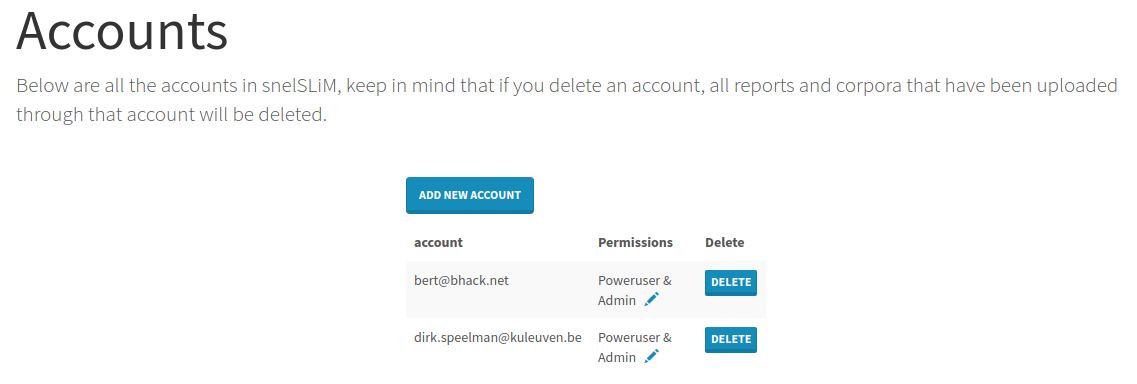
\includegraphics[width=0.9\textwidth]{images/users.png}}

\subsection{Global corpora}

On the ``My corpora'' page, admins don't just see their own corpora but have a distinction between global and personal corpora. After uploading corpora, they can promote them to global corpora available to every account, as well as delete global corpora that may have been replaced or are no longer relevant.

\centerline{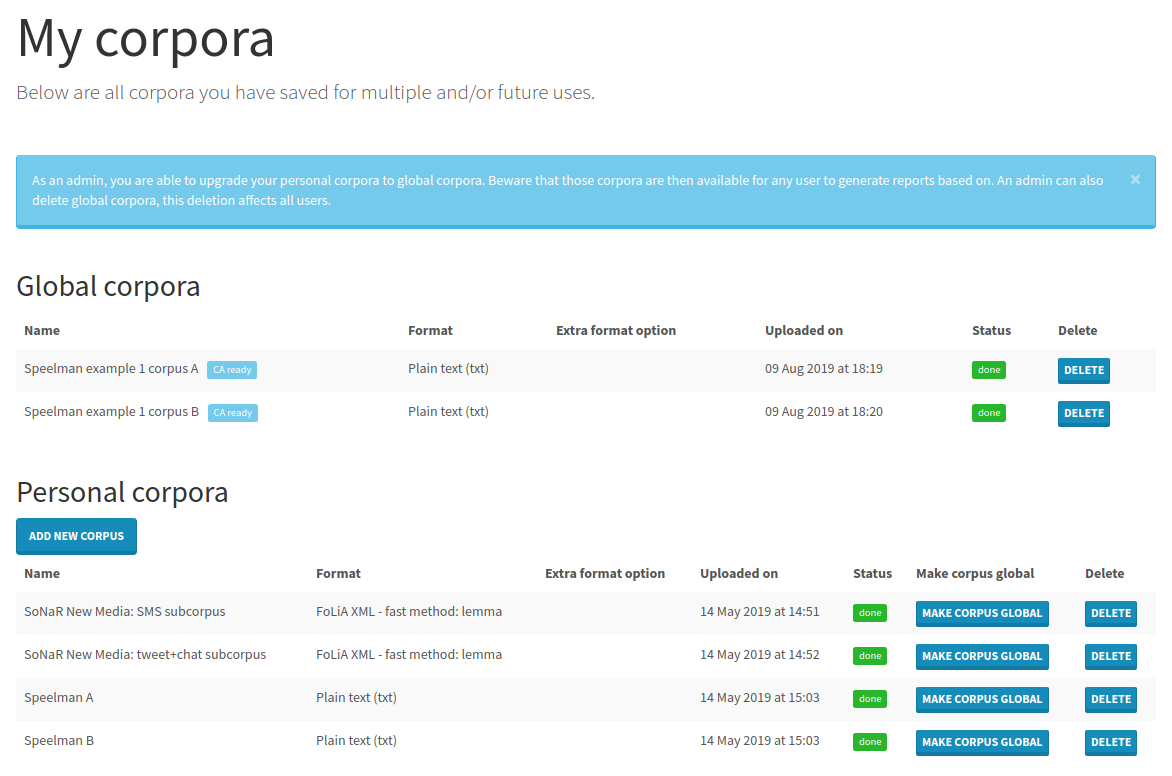
\includegraphics[width=0.9\textwidth]{images/admincorpora.png}}

\section{Installer/System administrator settings}

As part of the installation, system administrators are not only required to configure a database, but also to set some application settings within the config.php file. If any problems arise where you as a user are not correctly receiving email notifications that your reports have finished, are unable to increase the amount of frequent items to be analysed to the desired number, or hitting time out when supplying temporary corpora, these are all settings that the system administrator has control over. You can contact him or her explaining your issues. They should be able to rectify them by tweaking the config.php applications settings as described in the installation guide they used to install snelSLiM. 

\section{Issues and feature requests}

If you are experiencing issues that are not related to your corpus or installation but originate from a specific problem with snelSliM, as well as if you have specific feature requests to further extend the functionality, usability or user friendliness of snelSLiM, you are free to submit detailed explanation through a GitHub issue on \url{https://github.com/bertvandepoel/snelSLiM/issues}. Please do make sure no one else has already submitted your issue or request before posting.

\end{document}